\documentclass[letterpaper]{scrartcl} % nicer style than 'article'
\usepackage[utf8]{inputenc}
\usepackage[english]{babel}
\usepackage[backend=biber,
	style=authoryear,
	doi=false,url=false,isbn=false,
maxcitenames=3]{biblatex}

% hyperref creates pdf metadata, including table of contents
\usepackage{caption,subcaption,verbatim,amsmath,amssymb,amsthm,graphicx,hyperref}
\usepackage[dvipsnames]{xcolor}

\graphicspath{{graphics/}} % where to look for image files
\addbibresource{tex/references.bib} % separate file for bibtex references
\AtEveryBibitem{\clearlist{language}} % clears language from bib entries

% define what you need
\newtheorem{proposition}{Proposition}
\newtheorem{lemma}{Lemma}
\newtheorem{claim}{Claim}

% define some variables for reuse
\newcommand{\mytitle}{Article Title}
\newcommand{\mysubtitle}{Article Subtitle}
\newcommand{\myname}{Toban Wiebe}

\hypersetup{% set up hyperref to generate pdf metadata
	pdftitle={\mytitle},
	pdfauthor={\myname},
}

% comment out fields you don't want
\title{\mytitle}
\subtitle{\mysubtitle}
\author{\myname}
\date{\today}


\begin{document}

\maketitle % generate title page

% modular contents
%!TEX root = ../main.tex

\begin{abstract}
	This is the abstract of the paper.
	Maybe there's some math in it: \( \mathbb E [X] = \int x dF \).
	Lorem ipsum dolor sit amet, sed fabellas salutatus voluptatum ei, feugiat ornatus singulis pro ut.
	Rebum iuvaret concludaturque mei no, et putent propriae has.
	Eum ei dolorem voluptaria intellegebat, te mei mollis theophrastus, vim ne hinc magna appareat.
	Audiam accusam ad mei, nibh meis vim ne.
\end{abstract}
 % for a page break, use \newpage
%!TEX root = main.tex

\section{Introduction}

Lorem ipsum dolor sit amet, vis id dolores albucius perfecto, ex mel unum vidit voluptatibus, altera phaedrum mea ut.
Latine docendi mel ei, inermis delicata cu vis.
No pertinax iudicabit usu, vis molestie corrumpit ex.
Pri cu oblique legendos, an nullam meliore reformidans sed.
Quo id ferri lobortis.

Cu est deleniti cotidieque.
An ius enim legimus praesent, eu wisi adipiscing vel.
Sale dolor necessitatibus eu mel, hinc fabulas necessitatibus ne pro.
At facete hendrerit sit, labores repudiandae ullamcorper id vix.

%!TEX root = ../main.tex

\section{Literature}

Citing some papers \textcite{axelrod1981evolution} and \textcite{rothschild1976equilibrium}.

%!TEX root = ../main.tex

\section{Model}

The Standard Normal~\footnote{See Claim~\ref{clm:example}.} distribution has density function \( \phi(x) = \frac{1}{\sqrt{2 \pi}} e^{-\frac{x^2}{2}} \) and distribution function
\[
	\Phi(x) = \frac{1}{\sqrt{2 \pi}} \int_{-\infty}^x e^{-\frac{s^2}{2}}ds.
\]

\begin{comment}
This is a multiline or block comment.
The `comment` environment is provided by the `verbatim` package.

All this stuff is just ignored.
\end{comment}

%!TEX root = ../main.tex

\section{Results}

Figure~\ref{fig:equilibrium} shows the equilibrium.

\begin{figure}
	\centering
	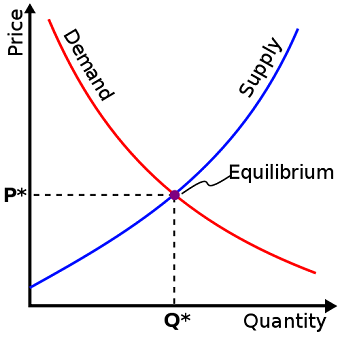
\includegraphics[width=0.6\textwidth]{supply-demand-equilibrium.png}
	\caption{The results}
	\label{fig:equilibrium}
\end{figure}


\printbibliography{} % insert references

%!TEX root = main.tex

\section{Appendix}

\begin{claim}
	Stuff goes here.
	\label{clm:example}
\end{claim}

\begin{proof}
	Because I said so.
\end{proof}


\end{document}
